\RequirePackage[l2tabu, orthodox,abort]{nag}

\InputIfFileExists{jfsettings}{}{
  \documentclass[12pt,oneside,reqno]{amsart}
  \usepackage[a4paper,portrait,left=1.5cm,outer=3.5cm,headheight=15pt,bottom=3cm,top=3cm]{geometry}
}

%%%%%%%%%%%%%%%%%%%%%%%%%%%%%%%%%%%%%%%%%%%%%%%%%%%%%%%%%%%%%%%&
% Draft settings
\usepackage{xcolor}
\usepackage[color]{showkeys}
\definecolor{refkey}{rgb}{0.3,0.5,0.3}
\definecolor{labelkey}{rgb}{0.3,0.5,0.3}
\definecolor{todo}{rgb}{0.6,0.9,0.5}
\usepackage[textwidth=3cm,textsize=tiny,color=todo]{todonotes}
\usepackage{hyperref}

%%%%%%%%%%%%%%%%%%%%%%%%%%%%%%%%%%%%%%%%%%%%%%%%%%%%%%%%%%%%%%%%%
%%  GENERAL SETTINGS

\usepackage{amsmath,amssymb,amsfonts,amsthm} % ams stuff everywhere
\usepackage{array}                 % math in tabular etc.
\usepackage{booktabs}              % improve table rendering
\usepackage[utf8]{inputenc}        % UTF8 fonts
\usepackage[T1]{fontenc}           % Fix font encoding issues with accented chars
\usepackage[english]{babel}        % Language awareness
\usepackage{csquotes}              % Context sensitive qouting
\usepackage{enumitem}              % no dull items
\usepackage{tikz}
\usepackage{verbatim}
\usepackage{graphicx}
\usepackage{fouriernc}
\usepackage[amssymb,thickspace,thinqspace]{SIunits}

\graphicspath{ {./} {./pic/}}
\numberwithin{equation}{section}




\title[Numerical solution of Generalized Nernst-Planck-Poisson (Draft)]{Numerical solution of Generalized Nernst-Planck-Poisson systems\\ Draft}

\author{$\dots$}
\date{\today}



\begin{document}
\maketitle

\section{Introduction}

The authors of \cite{dreyer2013overcoming,dreyer2014mixture,guhlke2015theorie,dreyer2016new} provide a thermodynamically and  mathematically motivated  derivation of Generalized Nernst-Planck-Poisson systems and Butler-Volmer - like  electrochemical reaction equations  assuming
\begin{itemize}
  \item ions in electrolytes have finite sizes and are solvated,
  \item electrode reactions take place at the interface between the electrolyte and the electrode metal,
  \item in a boundary layer defined by the plane of zero charge, short relaxation times allow the assumption that the electrochemical potential of the dissolved species is constant.
\end{itemize}

This paper describes a finite volume discretization approach of the resulting generalized Poisson-Nernst-Planck system based on the excess chemical potential scheme described and investigated in \cite{liu2014poisson, CCFG2021, GaudeulFuhrmannNM2022} and appearantly first introduced in \cite{SEDAN}.
%
It describes the link between electrode boundary conditions for the generalized Nernst-Planck-Poisson system assuming electrochemical reactions at the metal-electrolyte interface and a Butler-Volmer-like boundary condition for the Nernst-Planck system with local electroneutrality derived by using the method of matched asymptotics in \cite{guhlke2015theorie,dreyer2016new}.
%
Using the finite volume discretization approach, the paper provides a numerical assessment of the this connection for a simple redox reaction.

%%%%%%%%%%%%%%%%%%%%%%%%%%%%%%%%%%%%%%%%%%%%%%%%%%%%%%%%%%%%
\section{A Generalized Poisson-Nernst-Planck system}
See e.g. \cite{wang2013simulations} and references cited therein.
\begin{subequations}\label{sys:PNPgamma}
  \begin{align}
    -\nabla \varepsilon \nabla \phi            & = q \label{eq:Poisson}                                                                                                                    \\
    \partial_t c_i  + \nabla \cdot \mathbf N_i & =0                                                                                                      & (i=1\dots N)                    \\
    \mathbf N_i                                & =-D_i c_i \left( \nabla\log \left(\gamma_i\frac{c_i}{c^\circ}\right) + z_i\frac{F}{RT}\nabla\phi\right) & (i=1\dots N) \label{eq:NPgamma}
  \end{align}
\end{subequations}
For the notations, see Table \ref{tab:notations}. The unknown scalar fields to be determined are the concentrations $c_i$ and
the electrostatic potential $\phi$. The activity coefficients $\gamma_i$ describe the deviation from the unmodified
Nernst-Planck flux (where $\gamma_i=1$), as one can see from the equivalent flux expression based on the excess chemical potential $\mu_i^{ex} =  RT \log \gamma_i$:
\begin{align}
  N_i= -D_i\nabla c_i  - \frac{D_i}{RT} c_i(\nabla\mu^i_{ex} +z_iF\nabla\phi) \label{eq:exflux}.
\end{align}
This  in generalized drift-diffusion form
combines an essentially Fickian diffusion term with a drift term combining the gradients of the electrostatic potential and the excess chemical potential.


\begin{table}
  \begin{tabular}{r@{:~~}l}
    $\phi $ & electrostatic potential    \\
    $p$     & pressure                   \\
    $\mu_i$ & species chemical potential \\
    $c_i$   & molar concentration        \\
    $N_i$   & molar flux                 \\
    $z_i$   & species charge number      \\
    $D_i$   & diffusion coefficient      \\
    $v_i$   & molar volume               \\
  \end{tabular}
  \begin{tabular}{r@{:~~}l}
    $M_i$         & species molar mass                   \\
    $\kappa_i$    & species solvation number             \\
    $\mu_i^\circ$ & species reference chemical potential \\
    $p^\circ$     & reference pressure                   \\
    $\varepsilon$ & dielectric constant                  \\
    $F$           & Faraday constant                     \\
    $R$           & molar gas constant                   \\
    $T$           & temperature                          \\
  \end{tabular}

  \begin{tabular}{r@{:~~}l}
    $  \bar c = \sum_{i=0}^N  c_i$                             & molar concentration of mixture   \\
    $q=F\sum_{i=1}^N z_i c_i$                                  & electric charge density          \\
    $\bar v_i = v_i + \kappa_i v_0$                            & solvated molar volume            \\
    $m_i=\frac{M_i+\kappa_iM_0}{M_0}=\frac{M_i}{M_0}+\kappa_i$ & solvated molar mass ratio        \\
    $c^\circ = \frac{1}{v_0}$                                  & constant reference concentration
  \end{tabular}
  \medskip

  \caption{Notations}
  \label{tab:notations}
\end{table}

\subsection{Gouy-Chapman model}
This corresponds to the unmodified Poisson-Nernst-Planck-System.
It assumes
\begin{align}
  \label{eq:gc}
  \gamma_i   & =1  \\
  \mu_i^{ex} & =0.
\end{align}



\subsection{Bikerman-Freise model}
Assuming, that all ions and the solvent molecules have the same molar volume $v_0$, and that they fill up
the available volume: $v_0\sum_{i=0}^N c_i = 1$, we set
\begin{align}
  \gamma_i   & =\frac{1}{v_0c_0}= \frac{1}{1-v_0\sum_{i=1}^N c_i} \\
  \mu_i^{ex} & = -RT\log(v_0c_0)
\end{align}

\subsection{Extended Bikerman-Freise model:} \cite{ringe2020double, wang2013simulations} and references therein.
This model is similar to the previous one, but assumes species filling up the available space
with different species molar volumes $v_i$: $\sum_{i=0}^N v_ic_i = 1$.
\begin{align}
  \gamma_i   & = \frac{1}{v_0c_0} = \frac{1}{1-\sum_{j1}^N v_j c_j} \\ \label{eq:XBF}
  \mu_i^{ex} & = -RT\log(v_0c_0)
\end{align}

\subsection{Calculation from chemical potential functions}
Assume we are given chemical potential functions $\mu_i$ $(i=0\dots N)$ depending
on concentrations, pressure or any other variables. The general schem to calculate the
excess chemical potential and the activity coefficients is as follows:

According to \cite{dreyer2014mixture,FuhrmannFuelCells2016},

\begin{align}
  \mathbf N_i & = - \frac{D_i}{RT} c_i \left( \nabla \mu_i - m_i\nabla \mu_0 + z_i F \nabla \phi \right). & (i=1\dots N) \label{eq:NP}
\end{align}
Therefore,
\begin{align}\label{eq:muexdef}
  \mu^{ex}_i & = \mu_i - m_i\mu_0 -  RT \log \frac{c_i}{c^\circ}, & (i=1\dots N)
\end{align}
where $c^\circ$ is some constant reference concentration.
Then, if we choose $c^\circ=\frac{1}{v_0}$, the concentration of the solvent without ion content,
\begin{align}
  \gamma_i= \exp\left(\frac{\mu^{ex}_i}{RT}\right)
  = \frac{\exp{\left(\frac{\mu_i - m_i\mu_0}{RT}\right)}}{c_iv_0}
\end{align}

Equation \eqref{eq:NP} describes three forces influencing the movement of ionic species: the gradient of the species chemical potential $\mu_i$, the gradient of the electrostatic potential $\phi$ and the negative gradient of the solvent chemical potential $\mu_0$.
%
In essence, the later takes into account the energy needed to displace solvent molecules when an ion moves, paying attention to the fact that ions and solvent molecules have finite (nonzero) sizes.
%
As a consequence, only a limited number of them fit into a given volume.
\subsection{DGML model}

Chemical potentials, concentrations and pressure are related via \cite{dreyer2013overcoming,dreyer2014mixture}:
\begin{align}\label{eq:constrel}
  \mu_i & = \mu_i^\circ + \bar v_i(p-p^\circ) + RT \ln \frac{c_i}{\bar c}. & (i=0\dots N),
\end{align}
where $\bar v_i$ is the solvated molar volume.
%
Asuming mechanical equilibrium conditions and zero barycentric velocity reduces the momentum balance $p$ to the relationship $\nabla p = q \nabla \phi$.
%
We have the orthogonal Helmholtz decomposition of $F= \nabla p - q \nabla \phi = \nabla \psi + W$  where $\psi$ is some scalar function defined by $\Delta \psi = \nabla \cdot F$, and $W$ is a solenidal vector field with $\nabla\cdot W =0$.
Assuming in addition that the gradient of the charge density $\nabla q$ is parallel to the electric field $-\nabla \phi$, we have that $\nabla\times W = \nabla\times  (q \nabla \phi) = \nabla q \times \nabla \phi = 0$, and thus $W=0$.
%
This allows to replace the momentum balance relationship by \cite{Fuhrmann2015}:
\begin{align}
  -\Delta p + \nabla \cdot q \nabla \phi = 0 \label{eq:press}
\end{align}


The system is closed by the incompressibility condition
\begin{align}\label{eq:incompress}
  \sum_{i=0}^N \bar v_ic_i & =1.
\end{align}
%
By \eqref{eq:incompress} one can obtain the solvent concentration $c_0$  from the solute concentrations
$c_1\dots c_N$:
\begin{align}
  \label{eq:c0}
  c_0 & =\frac{1}{v_0} -  \sum_{i=1}^N  \frac{\bar v_i}{v_0}c_i
\end{align}

For $i=1\dots N$ one has, omitting constant terms not relevant for the gradient:
\begin{align}
  \mu_i^{ex} & = \mu_i -m_i \mu_0  - RT \log (v_0c_i)\nonumber                                                                                \\
             & = \bar v_ip +  RT \log \frac{c_i}{\bar c}  -m_i\left(  v_0p + RT \log \frac{c_0}{\bar c}\right)  - RT \log (v_0c_i)  \nonumber \\
             & = \bar v_ip - RT\log v_0\bar c -m_i\left(v_0p + RT \log \frac{c_0}{\bar c}\right)\nonumber                                     \\
             & = \left(\bar v_i-m_iv_0\right)p -m_iRT\log \frac{c_0}{\bar c} - RT\log v_0 \bar c. \label{eq:muex}
\end{align}
Express $c_0$ via \eqref{eq:c0} and $\bar c$ in terms of $c_1\dots c_N$:
%
\begin{align*}
  \bar c & % = \frac{1}{v_0} -  \sum_{i=1}^N \frac{\bar v_i}{v_0}c_i + \sum_{i=1}^N  c_i
  = \frac{1}{v_0} + \sum_{i=1}^N \left(1- \frac{\bar v_i}{v_0}\right) c_i .
\end{align*}
%
The corresponding activity coefficient is
\begin{align}
  \gamma_i(c_1\dots c_N, p) & =\exp\left(\frac{\mu_i^{ex}}{RT}\right)
  = \frac{1}{v_0\bar c}\exp\left(\frac{\bar v_i-m_iv_0}{RT}p\right)\left(\frac{\bar c}{c_0}\right)^{m_i}. \label{eq:gamma}
\end{align}

\subsection{Constant density model}: \cite{FGLMMSpringer2019}
The density of the mixture is
\begin{align*}
  \rho & = M_0 c_0 + \sum_{i=1}^N (M_i + \kappa_i M_0) c_i
  %  = M_0\frac{1}{v_0} -  \sum_{i=1}^N  M_0\frac{\bar v_i}{v_0}c_i + \sum_{i=1}^N (M_i + \kappa_i M_0) c_i\\
  = M_0\frac{1}{v_0} -  \sum_{i=1}^N  \left(M_i + \kappa_i M_0 - M_0\frac{\bar v_i}{v_0}\right)c_i .
\end{align*}
The density $\rho$ remains constant if $m_i=\frac{M_i + \kappa_i M_0}{M_0} = \frac{\bar v_i}{v_0}$,
leading to
\begin{align}
  \gamma_i   = \frac{1}{v_0\bar c}\left(\frac{\bar c}{c_0}\right)^{\frac{\bar v_i}{v_0}}
\end{align}
independent of the pressure $p$.


This model is relevant as a simplification allowing to couple to Navier-Stokes solvers which assume constant density of the fluid.


\subsection{Domain, boundary and initial conditions}\label{sec:bc}
For the subsequent discussion and the numerical example, we assume a simple model half cell  in the domain $(0,L)$ with  a working electrode at  $x=0$  and  a bulk interface at  $x=L$. This approach can be generalized to more complicated geometrical configurations.

Assume Dirichlet boundary conditions $\phi|_{x=L}=0, p|_{x=L}=0, c_i|_{x=L}=c_i^{bulk}$
at the bulk interface $x=L$, such that electroneutrality $\sum_{i=1}^N z_ic_i^{bulk}=0$ is fulfilled and $c_0^{bulk}>0$.
Applying a potential at the working electrode leads to  a  Dirichlet boundary condition
for the electrostatic potential:
\begin{subequations}\label{sys:PNPbc}
  \begin{align}\label{eq:PNPpot}
    \phi|_{x=0}=U.
  \end{align}
  For the pressure at the electrode,  set a ``do nothing'' boundary condition
  \begin{align}
    (\nabla p - q\nabla \phi)\cdot \vec n|_{x=0}=0.
  \end{align}
  %
  For the constituents of the electrolyte  assume a balance between normal fluxes and surface reactions, where
  $\mu_i^S$ are the species chemical potential at the surface.
  \begin{align}
    (N_i\cdot \mathbf n)|_{x=0} & =R_i(\mu_0^S\dots\mu_n^S), & (i=1\dots N)
  \end{align}
  Particular expressions will be discussed later. In addition to the chemical potentials
  of the dissolved species, $R_i$ depend on the electron concentration in the metal
  which is assumed to be constant and thus can be hidden in the constants describing $R_i$.
  Assuming that surface and bulk chemical potentials are equal leads to the equivalences
  \begin{align*}
    \mu_i^S=\mu_i|_{x=0}.
  \end{align*}
\end{subequations}
As initial conditions, we set $\phi|_{t=0}=0$, $p|_{t=0}=0$  $c_i|_{t=0}=c_i^{bulk}$ ($i=1\dots N$).

%%%%%%%%%%%%%%%%%%%%%%%%%%%%%%%%%%%%%%%%%%%%%%%%%%%%%%%%%%%%%%%%
\section{Draft: Susceptibility}
\begin{align*}
  \chi= \chi(c_0\dots c_n) = \chi_a(|E|^2)  + \chi_m(c_0\dots c_n, |E|^2)= \chi_a(|E|^2) +  \sum_{i=0}^n c_i \bar v_i\chi_i(|E|^2) 
\end{align*}
where $E=\nabla \phi$ is the electric field.

This gives an additional contribution to the chemical potential
\begin{align*}
  \mu_i^{pol}= -\bar v_i\frac{\varepsilon_0}{2}\chi_i(|E|^2)
\end{align*}
and the pressure condition becomes

\begin{align*}
  \nabla p = q\nabla \phi + \chi_m (\nabla E) \cdot \varepsilon_0 E
\end{align*}

Taking the divergence yields for 1D
\begin{align*}
  -\Delta p + \nabla \cdot q\nabla \phi + \nabla \cdot (\chi_m \psi  \varepsilon_0 \nabla \phi) & =0\\
  -\Delta \phi +\psi &= 0
\end{align*}

In the higher dimensional case we need a good reconstruction  of  $\nabla \phi$

%%%%%%%%%%%%%%%%%%%%%%%%%%%%%%%%%%%%%%%%%%%%%%%%%%%%%%%%%%%%%%%%
\section{Thermodynamic equilibrium problem}\label{sec:equilibrium}
Zero flux and integrating \eqref{eq:gammaflux} gives:
\begin{align*}
  \log (\gamma_iv_0c_i) + z_i\frac{F}{RT}\phi & = C \\
  \gamma_iv_0c_i\exp(z_i\frac{F}{RT}\phi)     & = K \\
  \gamma_ic_iv_0= K\exp(-z_i\frac{F}{RT}\phi)
\end{align*}
Assuming the existence of a bulk reference concentration $c_i^b$ at a potential $\phi^b$ and pressure $p^b$ allows
to define $K$:
\begin{align*}
  \gamma_i^bc_i^bv_0 & = K\exp\left(-z_i\frac{F}{RT}\phi^b\right)                 \\
  K                  & = \gamma_i^bc_i^bv_0\exp\left(z_i\frac{F}{RT}\phi^b\right)
\end{align*}
Thus,
\begin{align}
  \gamma_ic_iv_0 & = \gamma_i^bc_i^bv_0 \exp\left(z_i\frac{F}{RT}(\phi^b-\phi)\right)                             \\
  c_i            & = c_i^b\frac{\gamma_i^b}{\gamma_i}\exp\left(z_i\frac{F}{RT}(\phi^b-\phi)\right) \label{eq:pbc}
\end{align}
For  a general activity coefficient function $\gamma_i = \gamma_i(c_1\dots c_N, p)$, for given $\phi, p$, this
is an algebraic system determining the concentration $c_i$.

As a consequence, the equilibrium problem consists of the Poisson equation \eqref{eq:Poisson}, the modified momentum balance \eqref{eq:press} and the algebraic condition \eqref{eq:pbc}. In general, \eqref{eq:pbc} couples all species concentrations, so this equation needs to be made part of the nonlinear system to be solved.

The resulting concentration, and therefore the charge density become functions of $p$ and $\phi$.

In this case, the assumption that $\nabla q \parallel \nabla \phi$ follows directly from the momentum balance.

With  corresponding coefficients,  \eqref{eq:pbc} decouples and becomes independent of the pressure. In that case, concentrations, and therefore space charge densitiy can be calculated directly from the electric potential, thus reducing the eqilibrium system to a generalized Poisson-Boltzmann problem.



%%%%%%%%%%%%%%%%%%%%%%%%%%%%%%%%%%%%%%%%%%%%%%%%%%%%%%%%%%%%%%%%%%%%%%%%%%%%%%%%%%%%%%%%%%%%%%%%
\subsection{Electroneutral Nernst-Planck   system}
For  large  domains, the  width  of  the polarization  boundary  layer inherent to  the NPP-System is  very small, and it makes sense  to replace the Poisson equation with the local electroneutrality constraint:
\begin{align}
  0 & = \sum_{i=1}^N z_i c_i \label{eq:eneu}
\end{align}
%
This condition can be enforced just by setting  $\varepsilon=0.$
%
As the Poisson equation is replaced by an algebraic condition, the Dirichlet boundary conditions for the electrostatic potential at the electrode is removed, but  the reaction boundary conditions are kept.:
\begin{subequations}\label{sys:NNPbc}
  \begin{align}\
    (N_i\cdot \mathbf n)|_{x=0} & =R_i(\mu_0^S\dots\mu_n^S). & (i=1\dots N)
  \end{align}
\end{subequations}

In \cite{guhlke2015theorie,dreyer2016new}, based on an approach introduced in \cite{caginalp1988dynamics}, the method of matching asymptotic expansions has been used  to derive boundary conditions for this case.
%
As a main conclusion, the assumption of local equilibrium  in the polarization boundary layer is valid and  the electrochemical potentials $\mu_i + z_i F \phi$ are constant in this boundary layer.
%
A similar analysis already was performed in \cite{rubinstein1990electro}, albeit without the connection to the Butler-Volmer equation.
%
Assuming that the electrostatic potential at the metal side of the electrode at $x=0$ still assumes the applied potential value $U$, the potential difference over the polarization boundary layer can be expressed as $\phi(0)-U$, allowing to calculate the chemical potentials at the surface entering \eqref{sys:NNPbc} as
\begin{subequations}\label{sys:neubc}
  \begin{align}
    \mu_i^S=\mu_i(0) + z_i F(\phi(0)-U)
  \end{align}
\end{subequations}

The pressure equation \eqref{eq:press} has a zero right hand side leading to a constant value of the pressure with the boundary conditions involved.


\subsection{Surface reaction terms}
\cite{dreyer2016new, MuellerPersonal}
Assume equality of surface and bulk chemical potentials, and that the only species on the metal side are electrons which are given the index $-1$.

Let $A_0\dots A_N$ be the reacting species. Then one can write a (surface) reaction $R_\nu$ as
\begin{align}
  \sum_{i=-1}^N a_{\nu,i} A_i
  \begin{array}{c}
    k_\nu^+            \\
    \leftrightharpoons \\
    k_\nu^-            \\
  \end{array}
  \sum_{i=-1}^N b_{\nu,i} A_i.
\end{align}
Mass and charge conservation yield for each $\nu$
\begin{align}
  \sum_{i=-1}^N M_i s_{\nu,i}=0, \qquad
  \sum_{i=-1}^N z_i s_{\nu,i}=0,
\end{align}
where $s_{\nu,i}=b_{\nu,i}-a_{\nu,i}$.
Thus, with $z_{-1}=-1$ and $n=s_{\nu,-1}$ is the number of electrons
transferred per reaction, we have
\begin{align}
  \sum_{i=0}^N z_i s_{\nu,i} & =s_{\nu,-1}=n
\end{align}
With the affinity
\begin{align}
  \mathcal A_\nu = \frac{1}{RT}\sum_{i=-1}^Ns_{\nu,i}\mu_i
\end{align}
one writes the rate expression as
\begin{align}\label{eq:rrate}
  \mathcal R_\nu(\mu_0\dots\mu_N)= k_{\nu,0}\left(\exp(-\alpha_\nu\mathcal A_\nu) - \exp((1-\alpha_\nu)\mathcal A_\nu)\right)
\end{align}
In the electroneutral case, one writes due to the equilibrium conditions in the boundary layer:
\begin{align}
  \mathcal A_\nu & = \frac{1}{RT}\left(\sum_{i=-1}^Ns_{\nu,i}\mu_i + \sum_{i=0}^Ns_{\nu,i}z_iF(\phi -U)\right)\nonumber \\
                 & = \frac{1}{RT}\left(n\mu_{-1}+ \sum_{i=0}^Ns_{\nu,i}\mu_i + nF(\phi -U)\right)\nonumber              \\
                 & = \frac{1}{RT}\left(\Delta g+ \sum_{i=0}^Ns_{\nu,i}\mu_i + nF(\phi -U)\right).
\end{align}
The last step assumes a constant chemical potential of the electrons which is turned into the parameter $\Delta g$.


%%%%%%%%%%%%%%%%%%%%%%%%%%%%%%%%%%%%%%%%%%%%%%%%%%%%%%%%%%%%%%%%%%%%%%%%%%%%%%%%%%%%%%%%%%%%%%%%
\section{Finite volume method and flux discretization}

A two point flux finite volume method on boundary conforming Delaunay meshes is used to approximate the problem.
%
It has been inspired by the successful Scharfetter-Gummel box method for the solution of charge transport problems in semiconductors \cite{ScharfetterGummel1969,bank1983numerical}.
%
For an overview on this method see \cite{farrell2017numerical}.
This method was initially developed for drift-diffusion problems in non-degenerate semiconductors.

The simulation domain $\Omega$ is partitioned into a finite number of closed convex polyhedral control volumes $K\in\mathcal K$ such that $K\cap L= \partial K\cap \partial L$ and $\overline\Omega=\bigcup_{K\in \mathcal K} K$.
%
With each control volume a node $\vec{x}_K\in K$ is associated. If the control volume intersects with the boundary $\partial \Omega$, its corresponding node shall be situated on the boundary: $\vec{x}_K\in\partial\Omega\cap K$.
%
The partition shall be \textit{admissible} \cite{EGH}, that is for two neighboring control volumes $K, L$, the \textit{edge} $\overline{\vec{x}_K\vec{x}_L}$ is orthogonal to the interface between the control volumes $\partial K \cap \partial L$.
%
Let $\vec h_{KL} = \vec x_L -\vec x_K$ and $h_{KL}=|\vec h_{KL}|$.
%
Then, the normal vectors to $\partial K$ can be calculated as $\vec n_{KL}=\frac1{h_{KL}}\vec h_{KL}$.


A constructive way to obtain such a partition is based on the creation of a boundary conforming Delaunay triangulation resp. tetrahedralization of the domain and the subsequent construction of its dual, the Voronoi tessellation intersected with the domain, see e.g. \cite{bank1983numerical,SiFuhrmannGaertner2010,farrell2017numerical}, see also Fig. \ref{fig:sgfv}.

The time axis is subdivided into intervals
\begin{align*}
  0=t^0< t^1 <\dots < t^{N_t}=t^\sharp.
\end{align*}

The general approach to derive a two point flux finite volume scheme for a conservation law
%
\begin{align*}
  %   \partial_t c_i + \nabla\cdot \vec J_i=0
  \partial_t c_i + \nabla\cdot \vec N_i=0
\end{align*}
%
consists in integrating the equation over a space-time control volume $K\times [t^{n-1},t^n]$:
%
\begin{align*}
  0= & \int\limits_{t^{n-1}}^{t^n} \int\limits_{K} (\partial_t c_i + \nabla\cdot \vec N_i)\ d\vec x\ dt
  =\int\limits_{t^{n-1}}^{t^n} \int\limits_{K}\partial_t c_i\ d\vec x\ dt +
  \int\limits_{t^{n-1}}^{t^n}\int\limits_{\partial K} \vec N_i \cdot \vec n\ ds\ dt                     \\
  =  & \int\limits_{K} (c_i^n-c_i^{n-1}) \ d\vec x  + \sum\limits_{\substack{L\; \text{neighbor}        \\\text{ of}\; K}}\ \int\limits_{t^{n-1}}^{t^n}\int\limits_{\partial K\cap \partial L}\vec N_i\cdot \vec n_{KL}\ ds \ dt\\
\end{align*}
Performing an unconditionaly stable implicit Euler time discretization, this is approximated via the discrete continuity eqution
\begin{align*}
  |K|\frac{c_{i,K}^n-c_{i,K}^{n-1}}{t^n-t^{n-1}}+
  \sum\limits_{\substack{L\; \text{neighbor of}\; K}}      |\partial K\cap\partial L| N^n_{i,KL}=0,
\end{align*}
%
and it remains to define the numerical fluxes $N^n_{i,KL}$ which should approximate the normal fluxes between two neighboring control volumes depending on the unknown values in the two collocation points $\vec x_K$ and $\vec x_L$ at moment $t^n$.

In the case $\mu_i^{ex}=0$, the classical Scharfetter-Gummel exponential fitting upwind scheme \cite{ScharfetterGummel1969}  developed in the context of semiconductor device simulation can be used. It is based on the idea to obtain the fluxes between two control volumes from the solution of a two point boundary value problem for \eqref{eq:NP} projected onto the edge $\vec x_K \vec x_L$ under given concentration values $c_{i,K}$ and $c_{i,L}$ and constant flux  \cite{ScharfetterGummel1969,EymardFuhrmannGaertner2006}.
The resulting flux expression is
\begin{align*}
  N^n_{i,KL}= D_i\frac{B(-z_i\delta\phi^n_{KL})c^n_{i,K} -B(z_i\delta\phi^n_{KL})c^n_{i,L}}{|\vec x_K -\vec x_L|},
\end{align*}
where $B(\xi)=\frac{\xi}{e^\xi-1}$ is the Bernoulli function, and $\delta\phi^n_{KL}= \frac{F}{RT}(\phi^n_K-\phi^n_L)$ is the electrostatic potential difference between  $\vec x_K$ and $\vec x_L$.


In the  generalized drift-diffusion representation \eqref{eq:flux} one observes that the gradient of the excess chemical potential acts on the species distribution in a similar way as the gradient of the electrostatic potential. This leads to the rather straightforward idea to define a generalized Scharfetter-Gummel flux approximating \eqref{eq:flux} as
\begin{align*}
  N^n_{i,KL}= D_i\frac{B(- \delta\mu^{ex,n}_{i,KL} -z_i\delta\phi^n_{KL})c^n_{i,K} -B(\delta\mu^{ex,n}_{i,KL} +z_i\delta\phi^n_{KL})c^n_{i,L}}{|\vec x_K -\vec x_L|},
\end{align*}
where $\delta\mu^{ex,n}_{i,KL}=\frac{1}{D_iRT}(\mu^{ex,n}_{i,K}-\mu^{ex,n}_{i,L})$.
This approach can be traced back to the handling of Fermi statistics in the source code of the SEDANIII semiconductor simulator \cite{SEDAN}
and was independently introduced in \cite{liu2014poisson}. In \cite{GaudeulFuhrmannNM2022} (without pressure dependency) it has been shown to keep natural concentration constraints, to follow entropy principles and to converge.
The modification of the Scharfetter-Gummel scheme \cite{ScharfetterGummel1969} proposed in \cite{Fuhrmann2015,FuhrmannFuelCells2016,FGLMMSpringer2019} is based on a reformulation of \eqref{eq:NP} in species activities and has been found to be inferior to the excess chemical potential based approach \cite{CCFG2021}.

Due  to the admissibility condition, the normal component of the electric field can be approximated as
\begin{align*}
  E^n_{KL} & = \varepsilon\frac{\phi^n_K - \phi^n_L}{|\vec x_K -\vec x_L|}
\end{align*}
and the discretization of the Poisson equation \eqref{eq:Poisson} can be written as
\begin{align*}
  0 & =-\sum\limits_{L\; \text{neighbor of}\; K} |\partial K\cap\partial L| E^n_{KL} + |K|F\sum_{i=1}^N z_i. c^n_{i,K} \\
\end{align*}
A similar approach gives the discretization of \eqref{eq:press}, and for the generalized Poisson-Boltzmann problem arising in \ref{sec:equilibrium}.
%
The excess chemical potential flux scheme ensures that also at the discrete level, with boundary conditions ensuring equilibrium, the generalized Nernst-Planck-Poisson system is identical with the solution of the generalized Poisson-Boltzmann problem \cite{GaudeulFuhrmannNM2022}.

\begin{figure}
  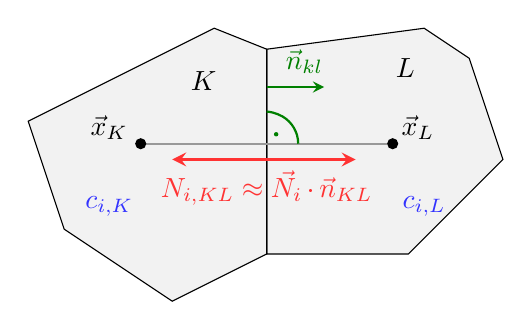
\begin{tikzpicture}[scale=0.8,>=stealth,shorten >=2pt]
    % \draw[step=1cm] (-4,-4) grid (8,4);
    \filldraw[fill=gray!10, draw=black]
    (2,1.5) --
    (4.5,1.83333) --
    (5.21429,1.35714) --
    (5.75,-0.25) --
    (4.25,-1.75) --
    (2,-1.75) --
    cycle;
    \filldraw[fill=gray!10, draw=black]
    (2,1.5) --
    (1.16667,1.83333) --
    (-1.78571,0.357143) --
    (-1.21429,-1.35714) --
    (0.5,-2.5) --
    (2,-1.75) --
    cycle;

    \draw[thick,gray!80] (0,0) -- (4,0);

    \draw (0,0) node[inner sep=0.5mm,shape=circle,fill] {} ;
    \draw (4,0) node[inner sep=0.5mm,shape=circle,fill] {} ;


    \draw (-0.5,0.25) node {$\vec{x}_K$};
    \draw (-0.5,-1) node {\textcolor{blue!80}{$c_{i,K}$}};


    \draw (4.4,0.25) node {$\vec{x}_L$};
    \draw (4.5,-1) node {\textcolor{blue!80}{$c_{i,L}$}};
    \draw[very thick,red!80,<->] (0.5,-0.25) -- (3.5,-0.25);
    \draw (2,-0.7) node {\textcolor{red!80}{$N_{i,KL}\approx \vec{N_i}\cdot\vec{n}_{KL} $}};


    % \draw (2.4,0.9) node {$\sigma_{kl}$};

    \draw (1,1) node {$K$};
    \draw (4.2,1.2) node {$L$};

    % \draw[thick,black,->] (1,-0.2) -- (3,-0.2);
    % \draw(1.5,-0.55) node {$\textcolor{black}{j_{k\ell}}$};

    \draw[green!50!black,thick,->] (2,0.9) -- (3,0.9);
    \draw(2.6,1.3) node {$\textcolor{green!50!black}{\vec{n}_{kl}}$};
    \draw [thick, green!50!black] (2.5,0) arc (0:100:0.5);
    \draw (2.15,0.15) node[very thick,green!50!black,inner sep=0.2mm,shape=circle,fill] {};
  \end{tikzpicture}
  \caption{Two neighboring control volumes}
  \label{fig:sgfv}
\end{figure}

\section{Numerical experiments}
\subsection{Implementation}
The method is implemented in the scientific computing programming language Julia based
on the VoronoiFVM.jl package for solving nonlinear systems of convection-diffusion-reaction
eaquations \cite{VoronoiFVM}. The implementation is provided in the Julia package LiquidElectrolytes.jl
\cite{LiquidElectrolytes}. The solution of the discretized nonlinear systems of equations is performed using
Newton's method with linearization by forward mode automatic differentiation \cite{revels2016forward}.

\subsection{Double layer capacitance}
Under the absence of a Faradaic reaction, the boundary condition for the ionic species
turns into a homogeneous Neumann boundary condition, and a steady state of the one-dimensional
system results in zero fluxes, and thus in thermodynamic equilibrium. A typical electrochemical
experiment is the calculation of the differential double layer capacitance. Given the bulk
local electroneutrality, the double layer charge can be calculated as $Q(U)=\int_0^L q dx$, where
$q$ is the right hand side of the Poisson equation  solved for an applied potential $u$.
The differential double layer capacitance then can be calculated as
\begin{align*}
  C_{dl}(U)= \frac{dQ}{dU} \approx  \frac{Q(U+h)-Q(U)}{h}
\end{align*}
Fig \ref{fig:dl} shows the double layer capacitances vs applied  potential for the
variation of the molarities and solvation numbers. The curves show the typical ``camel shape'' for
lower concentrations, and one observes a significant influence of the effective ion molar volume
on the capacitance maximum. The dots in the graphs denote the analytically calculated values
at the potential of zero charge, which is $0V$ in this case.
\begin{figure}
  \centering
  \includegraphics[width=0.45\textwidth]{example_dlcap_molvar.png}
  \includegraphics[width=0.45\textwidth]{example_dlcap_kappavar.png}
  \caption{Double layer capacitance for varying molarities (left) and varying solvation numbers (right)}
  \label{fig:dl}
\end{figure}

\subsection{Redox reaction: comparison between polarized and electroneutral cases}
Assume an aqeuous solution with reacting species
$O, R$  with charge numbers $z_O= z_R+n$.
%
Assume a redox reaction at the metal-electrolyte interface at $x=0$:
\begin{align}\label{eq:redox}
  O + ne^- & \rightleftharpoons R.
\end{align}
In the Poisson-Nernst-Planck (polarized) case, the discussions in section \ref{sec:bc} leads to the affinity
\begin{align*}
  \mathcal A= \frac{1}{RT}\left(\Delta g+ \mu_R - \mu_O\right)
\end{align*}
and the corresponding rate expression \eqref{eq:rrate}.

In the electroneutral Nernst-Planck system (obtained by setting $\varepsilon=0$) one arrives at
\begin{align*}
  \mathcal A= \frac{1}{RT}\left(\Delta g+ \mu_R - \mu_O+ nF(\phi -U)\right).
\end{align*}
This leads to
\begin{align}\label{eq:MBVneux}
  \mathcal R(\mu_O,\mu_R,\phi)= k_0\left(\exp\left(-\alpha\frac{\mu_R-\mu_O+nF(\phi-U)}{RT}\right)-\exp\left((1-\alpha)\frac{\mu_R-\mu_O+nF(\phi-U)}{RT}\right)\right).
\end{align}

Assuming the Bikerman-Freise model, the reaction rate expressed in concentrations is for $\alpha=\frac12$:
\begin{align}
  R_{redox}(c_O,c_R,\phi) & = k_0\left( \left(\frac{c_O}{c_R}\right)^{\frac12}\exp\left(\frac{zF(U-\phi)}{2RT}\right) - \left(\frac{c_R}{c_O}\right)^{\frac12}\exp\left(-\frac{zF(U-\phi)}{2RT}\right)\right) \\
                          & = \frac{\bar ck_0}{(c_Oc_R)^{\frac12}}\left(\exp\left(\frac{zF(U-\phi)}{2RT}\right)\frac{c_O}{\bar c} - \exp\left(-\frac{zF(U-\phi)}{2RT}\right)\frac{c_R}{\bar c}\right)
  \label{eq:MBVohm}
\end{align}
Replacing $\frac{\bar ck_0}{(c_Oc_R)^{\frac12}}$ by $j_0=\frac{\bar ck_0}{(c_O^\text{bulk}c_R^\text{bulk})^{\frac12}}$
yields a well known form of the Butler-Volmer equation \cite{BardFaulkner}.

In order to conform to typical experimental conditions, in addition to the redox species,  introduce an inert background electrolyte consisting of $X^+$ and cations $S^-$.
Adapt system \eqref{sys:PNP} and boundary conditions \eqref{sys:PNPbc} and regard the fluxes of the four species with the following boundary conditions
\begin{align*}
  \mathbf N_O|_{x=0} \cdot \vec n & = -\mathcal R & c_O|_{x=L}= c_O^{bulk} \\
  \mathbf N_R|_{x=0} \cdot \vec n & = \mathcal R  & c_R|_{x=L}= c_R^{bulk} \\
  \mathbf N_S|_{x=0} \cdot \vec n & = 0           & c_S|_{x=L}= c_S^{bulk} \\
  \mathbf N_X|_{x=0} \cdot \vec n & = 0           & c_X|_{x=L}= c_X^{bulk}
\end{align*}
where bulk electroneutrality is ensured: $z_Oc_O^{bulk}+z_Rc_R^{bulk}+z_Sc_S^{bulk}+z_Xc_X^{bulk}=0$.

\begin{figure}
  \centering
  \includegraphics[width=0.75\textwidth]{bvc_zr=-1.png}
  \caption{Steady state voltammetry curves for $z_R=-1, z_O=0$}
  \label{fig:zm1}
\end{figure}

\begin{figure}
  \centering
  \includegraphics[width=0.75\textwidth]{bvc_zr=0.png}
  \caption{Steady state voltammetry curves for $z_R=0, z_O=1$}
  \label{fig:z0}
\end{figure}

\begin{figure}
  \centering
  \includegraphics[width=0.75\textwidth]{bvc_zr=1.png}
  \caption{Steady state voltammetry curves for $z_R=1, z_O=2$}
  \label{fig:zp1}
\end{figure}

Figures \ref{fig:zm1} - \ref{fig:zp1} show the simulation results for steady state voltammetry -- solution
of the stationary system  with applied voltages $-1V \dots 1V$ -- for the polarized (PNP) and electroneutral (NNP) Nernst-Planck systems. In the region $-0.2V \dots 0.2V$ one observes a good coincidence of the currenents of both the polarized and the electroneutral cases, confirming the findings in \cite{guhlke2015theorie,dreyer2016new}.  Depending on species charges, when applying potential with equal polarity, one observes a breakdown of the current following a current peak due to electrostatic repulsion sometimes called ``Levich exclusion'' \cite{levich1949theory, dickinson2011influence}. Further current limitations in the polarized case compared to the electroneutral case are due to the accumulation of ions of the background electrolyte in the double layer. Finally, for large applied voltages, the current in the electroneutral case is transport limited due to the need of reactant diffusion to the electrode from the bulk end of the domain.

\bibliographystyle{unsrt}

\bibliography{description-literature}

\end{document}